% This file was converted to LaTeX by Writer2LaTeX ver. 1.0.2
% see http://writer2latex.sourceforge.net for more info
\documentclass[a4paper]{article}
\usepackage[utf8x]{inputenc}
\usepackage[T1]{fontenc}
\usepackage[spanish,english]{babel}
\usepackage{amsmath}
\usepackage{amssymb,amsfonts,textcomp}
\usepackage{color}
\usepackage{array}
\usepackage{hhline}
\usepackage{hyperref}
\hypersetup{pdftex, colorlinks=true, linkcolor=blue, citecolor=blue, filecolor=blue, urlcolor=blue, pdftitle=, pdfauthor=, pdfsubject=, pdfkeywords=}
\usepackage[pdftex]{graphicx}
% Outline numbering
\setcounter{secnumdepth}{0}
% List styles
\newcommand\liststyleLi{%
\renewcommand\labelitemi{{\textbullet}}
\renewcommand\labelitemii{${\circ}$}
\renewcommand\labelitemiii{${\blacksquare}$}
\renewcommand\labelitemiv{{\textbullet}}
}
\newcommand\liststyleLii{%
\renewcommand\labelitemi{{\textbullet}}
\renewcommand\labelitemii{${\circ}$}
\renewcommand\labelitemiii{${\blacksquare}$}
\renewcommand\labelitemiv{{\textbullet}}
}
\newcommand\liststyleLiii{%
\renewcommand\labelitemi{{\textbullet}}
\renewcommand\labelitemii{${\circ}$}
\renewcommand\labelitemiii{${\blacksquare}$}
\renewcommand\labelitemiv{{\textbullet}}
}
% Page layout (geometry)
\setlength\voffset{-1in}
\setlength\hoffset{-1in}
\setlength\topmargin{2cm}
\setlength\oddsidemargin{2cm}
\setlength\textheight{23.246668cm}
\setlength\textwidth{17.006cm}
\setlength\footskip{26.144882pt}
\setlength\headheight{1.016cm}
\setlength\headsep{0.508cm}
% Footnote rule
\setlength{\skip\footins}{0.119cm}
\renewcommand\footnoterule{\vspace*{-0.018cm}\setlength\leftskip{0pt}\setlength\rightskip{0pt plus 1fil}\noindent\textcolor{black}{\rule{0.25\columnwidth}{0.018cm}}\vspace*{0.101cm}}
% Pages styles
\makeatletter
\newcommand\ps@Standard{
  \renewcommand\@oddhead{{\raggedleft Introducción a la Computación -- Codificación de datos \ } {\raggedright \thepage{}}}
  \renewcommand\@evenhead{\@oddhead}
  \renewcommand\@oddfoot{}
  \renewcommand\@evenfoot{\@oddfoot}
  \renewcommand\thepage{\arabic{page}}
}
\makeatother
% \pagestyle{Standard}
\usepackage{fancyhdr}
\usepackage{sans}
\pagestyle{fancy}
% footnotes configuration
\makeatletter
\renewcommand\thefootnote{\arabic{footnote}}
\makeatother
\title{Codificación de Datos}
\author{Eduardo Grosclaude}
\date{2013-06-12}
\begin{document}

\section{Codificación de datos}
Hemos visto que la memoria de las modernas computadoras digitales está
diseñada para almacenar información en forma de bits, agrupados en
conjuntos de a ocho, y que cada una de estas unidades de ocho bits se
llama un byte. Usando la analogía natural entre valores de bits
(inactivo/activo) y dígitos binarios (0 o 1), hemos visto cómo la
memoria de una computadora digital moderna puede almacenar números no
negativos entre 0 y 255.

Sin embargo, los problemas de la vida real involucran otras clases de
datos. Muchos problemas requerirán manipular números mayores que
255, o números negativos, o con decimales; o aun, datos que no sean
numéricos, como texto, imágenes, sonido, o video. Si la única
manera posible de guardar contenidos en la memoria de la computadora es
en forma de bits, ¿cómo podremos manipular estas otras clases de
datos?

\subsubsection{Codificación de texto}
Cuando escribimos texto en nuestra computadora, estamos almacenando
temporariamente en la memoria una cierta secuencia de caracteres, que
son los símbolos que tipeamos en nuestro teclado. Estos caracteres
tienen una \textbf{representación gráfica} en nuestro teclado, en
la pantalla o en la impresora, pero mientras están en la memoria
\textbf{no pueden ser otra cosa que bytes}, es decir, conjuntos de ocho
dígitos binarios. Para lograr almacenar caracteres de texto
necesitamos adoptar una \textbf{codificación}, es decir, una tabla
que asigne a cada carácter un patrón de bits fijo.

Además, esta codificación debe ser \textbf{universal}: para poder
compartir información entre usuarios, o entre diferentes
aplicaciones, se requiere algún estándar que sea respetado por
todos los usuarios y las aplicaciones. Inicialmente se estableció con
este fin el \textbf{código
ASCII}\footnote{\url{http://es.wikipedia.org/wiki/ASCII}}, que durante
algún tiempo fue una buena solución. El código ASCII asigna
patrones de siete bits a un conjunto de caracteres que incluye:

\liststyleLi
\begin{itemize}
\item Las 25 letras del alfabeto inglés, mayúsculas y minúsculas; 
\item Los dígitos del 0 al 9, 
\item Varios símbolos matemáticos, de puntuación, etc., 
\item El espacio en blanco, 
\item Y 32 caracteres no imprimibles. Estos caracteres no imprimibles
son combinaciones de bits que no tienen una representación gráfica,
sino que sirven para diversas funciones de comunicación de las
computadoras con otros dispositivos. 
\end{itemize}
En general, prácticamente todos los símbolos que figuran en nuestro
teclado tienen un código ASCII asignado. Como sólo se usan siete
bits, el bit de mayor orden (el de más a la izquierda) de cada byte
siempre es cero, y por lo tanto los códigos ASCII toman valores de 0
a 127.

% \begin{center}
% \begin{figure}
% \begin{minipage}{17cm}
% 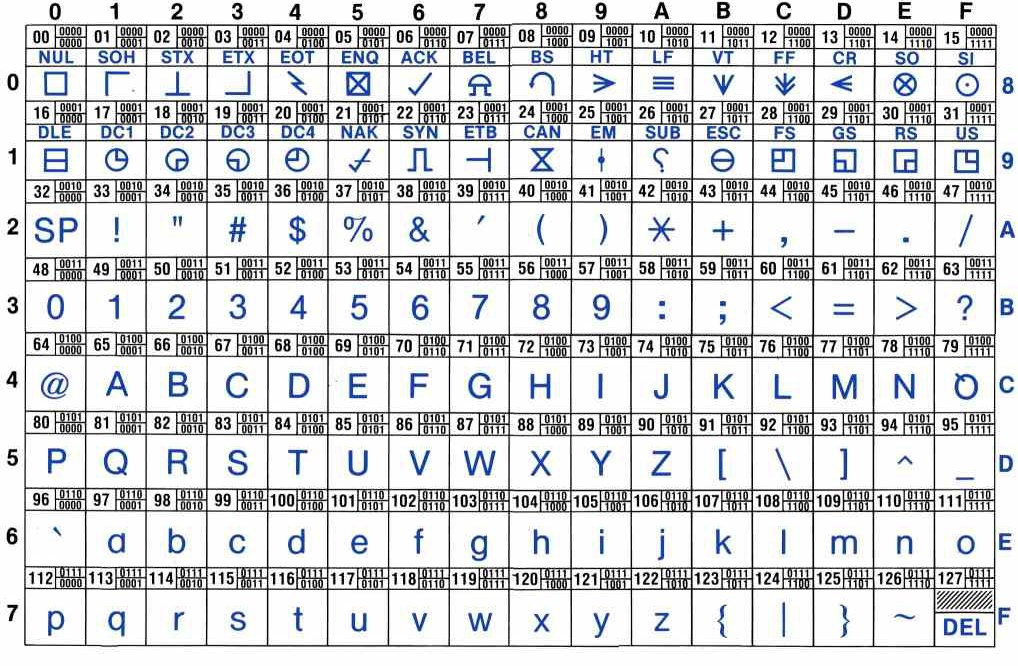
\includegraphics[width=13.335cm,height=9.423cm] {IC2020Codificacion20de20datos-img1.jpg}\end{minipage}
% {\centering\itshape
% Tabla ASCII, que codifica los caracteres más importantes\newline
% utilizando siete bits (el bit más significativo de cada ocho \newline es siempre cero).
% \par}
% \end{figure}
% \end{center}

%%% FRAMEBOX
%%% \begin{figure}
%%% \rule{\textwidth}{0.005in}
%%% \begin{center}\framebox{Fee Foe Fi Fum \ldots}\framebox{Fee Foe}\end{center}
%%% \caption{A very nice figure indeed}\label{very-nice-figure}
%%% \rule{\textwidth}{0.005in}
%%% \end{figure}

 \begin{figure}
 \begin{minipage}{17cm}
 \begin{center}
 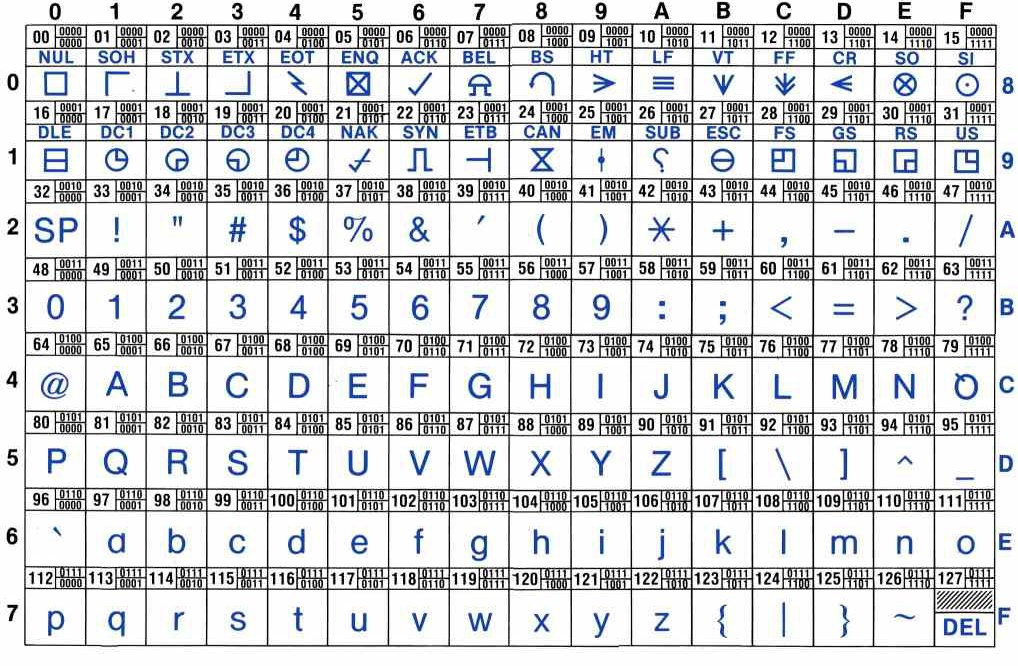
\includegraphics[width=13.335cm,height=9.423cm] {IC2020Codificacion20de20datos-img1.jpg}
 {\itshape  \par  Tabla ASCII, que codifica los caracteres más importantes utilizando siete bits \newline (el bit más significativo de cada ocho   es siempre cero).\par}
\rule{\textwidth}{0.005in}
 \end{center}
 \end{minipage}
 \end{figure}
Sin embargo, el código ASCII es insuficiente para muchas aplicaciones:
no contempla las necesidades de diversos idiomas. Por ejemplo, nuestra
letra \textbf{ñ} no figura en la tabla ASCII. Tampoco las vocales
acentuadas, ni con diéresis, como tampoco decenas de otros caracteres
de varios idiomas europeos. Peor aún, con solamente 256 posibles
patrones de bits, es imposible representar algunos idiomas orientales
como el chino, que utilizan miles de ideogramas.

Por este motivo se estableció más tarde una familia de nuevos
estándares, llamada
\textbf{Unicode}\footnote{\url{http://es.wikipedia.org/wiki/Unicode}}.
Uno de los estándares de codificación definidos por Unicode, el
más utilizado actualmente, se llama
\textbf{UTF-8}\footnote{\url{http://es.wikipedia.org/wiki/Utf-8}}. Este
estándar mantiene la codificación que ya empleaba el código ASCII
para ese conjunto de caracteres, pero agrega códigos de dos, tres y
cuatro bytes para otros símbolos. El resultado es que hoy, con UTF-8,
se pueden representar todos los caracteres de cualquier idioma
conocido.

\subsubsection{Codificación de multimedia}
Otras clases de datos, diferentes del texto, también requieren
codificación (porque siempre deben ser almacenados en la memoria en
forma de bits y bytes), pero su tratamiento es diferente. Introducir en
la computadora, por ejemplo, una \textbf{imagen analógica }(tal como
un dibujo o una pintura hecha a mano), o un fragmento de
\textbf{sonido} tomado del ambiente, requiere un proceso previo de
digitalización. \textbf{Digitalizar} es \textbf{convertir en digital}
la información que es \textbf{analógica}, es decir, convertir un
rango continuo de valores (lo que está en la naturaleza) a un
conjunto discreto de valores (que puede ser ingresado en la
computadora).

\paragraph[Imagen ]{Imagen }
En el caso de una imagen analógica, el proceso de digitalización
involucra la división de la imagen en una fina cuadrícula, donde
cada elemento de la cuadrícula abarca un pequeño sector
cuadrangular de la imagen. A cada pequeño sector, o elemento
cuadrangular, se le asignan valores discretos que codifican el color de
la imagen en ese lugar. Por ejemplo, se pueden asignar tres valores,
codificando la cantidad de rojo, de verde y de azul que contiene cada
lugar de la imagen. Luego cada uno de estos valores se puede expresar
como un entero. Si fuéramos a guardar cada uno de estos enteros en un
byte, quedaríamos limitados a valores entre 0 y 255. 

\liststyleLii
\begin{itemize}
\item Un elemento que fuera completamente rojo tendría valores (255,
0, 0). Un elemento de color verde puro tendría valores (0, 255, 0). 
\item Un elemento blanco tendrá los máximos valores para todos los
colores, que mezclados dan el color blanco: (255, 255, 255). 
\item Un elemento que es gris tendrá los tres valores aproximadamente
iguales pero menores que 255. 
\end{itemize}
En general, mientras más elementos podamos codificar, mejor será la
aproximación a nuestra pieza de información original. Mientras
más fina la cuadrícula (es decir, mientras mayor sea la
\textbf{resolución}\footnote{\url{http://es.wikipedia.org/wiki/Resolución\_de\_imágenes}}
de la imagen digitalizada), y mientras más valores discretos usemos
para representar los colores, más se parecerá nuestra versión
digital al original analógico.

Notemos que la digitalización de una imagen implica la
discretización de dos \textbf{variables analógicas}, o sea,
discretización en dos sentidos: por un lado, los infinitos puntos de
la imagen analógica, bidimensional, deben reducirse a unos pocos
rectángulos discretos. Por otro lado, los infinitos valores de color
deben reducirse a sólo tres coordenadas, con finitos valores en el
rango de nuestro esquema de codificación. Son dos ejemplos de
conversión de variables analógicas a digitales. Este proceso de
digitalización es el que hacen automáticamente una cámara de
fotos digital o un celular, almacenando luego los bytes que representan
la imagen tomada. Sin embargo, las modernas cámaras utilizan un
esquema de codificación con mucha mayor \textbf{profundidad de
color}\footnote{\url{http://es.wikipedia.org/wiki/Profundidad_de_color}}
(es decir, más bytes por cada coordenada de color) que en el ejemplo
anterior.


\bigskip



\begin{center}
\rule{\textwidth}{0.005in}
\begin{minipage}{17.006cm}
{\centering

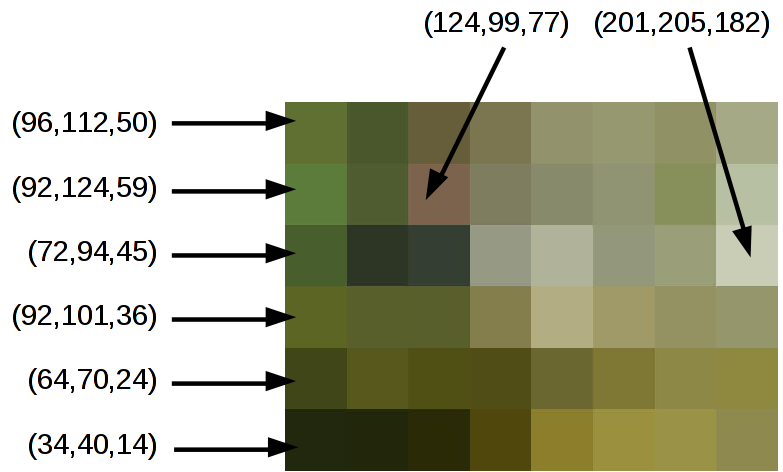
\includegraphics[width=8.375cm,height=5.048cm]{IC2020Codificacion20de20datos-img2.png}
 
\par}


\bigskip

{\centering\itshape
Imagen en baja resolución con 24 bits de profundidad de color.
\par}

\liststyleLiii
\begin{itemize}
\clearpage\item {\itshape
La primera columna tiene predominancia de verde (la segunda componente
es la mayor).}
\item {\itshape
Colores más oscuros tienen valores menores.}
\item {\itshape
El elemento que más tiende al rojo tiene la primera componente mayor.}
\item {\itshape
El elemento gris claro tiene las tres componentes aproximadamente
iguales, y de valor alto.}
\end{itemize}
\end{minipage}
\rule{\textwidth}{0.005in}
\end{center}
\clearpage

\begin{center}
\begin{minipage}{17cm}
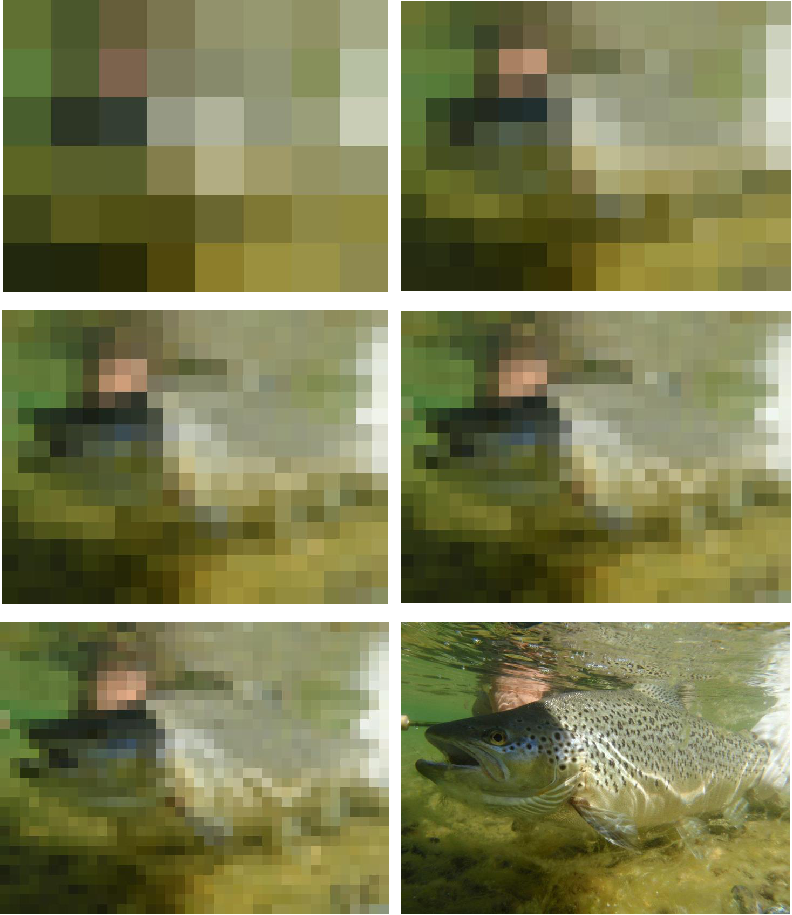
\includegraphics[width=15.309cm,height=17.687cm]{IC2020Codificacion20de20datos-img3.png}{\centering\itshape\par
La misma imagen digital, en varias resoluciones
\par}
\end{minipage}
\rule{\textwidth}{0.005in}
\end{center}

\subsubsection{Sonido}
En el caso del \textbf{sonido} (o \textbf{audio}), también tenemos dos
variables analógicas para digitalizar. Un micrófono actúa como un
\textbf{transductor}: traduce los impulsos físicos del sonido, que
llegan por el aire, a impulsos eléctricos. Necesitamos discretizar
esos impulsos eléctricos, y como en el caso anterior, esto ocurrirá
en dos sentidos. Por un lado, los impulsos eléctricos, provocados en
el micrófono por el sonido, ocupan un intervalo continuo de tiempo,
pero nos quedaremos sólo con unos cuantos valores por segundo. Por
otro lado, en cada intervalo de tiempo, los impulsos eléctricos
entregados por el micrófono ocupan un rango continuo de valores,
entre ciertos valores eléctricos extremos; pero necesitamos quedarnos
sólo con algunos valores enteros en ese rango. 

Nuevamente, mientras más muestras por segundo y más valores
diferentes reconozcamos en el rango de entrada, mejor se aproximará
nuestra digitalización del sonido al original (ver figura).
Aproximadamente así funcionan al captar nuestra voz los celulares,
una cámara filmadora digital, o un programa de grabación de sonido
que usamos en nuestra computadora. El resultado es una secuencia de
bytes que codifican el sonido que ingresó por el micrófono.


\bigskip



\begin{center}
\begin{minipage}{17cm}



{\raggedleft\itshape
Digitalización de un ciclo de una \newline
onda sonora en 16 niveles.
\par}


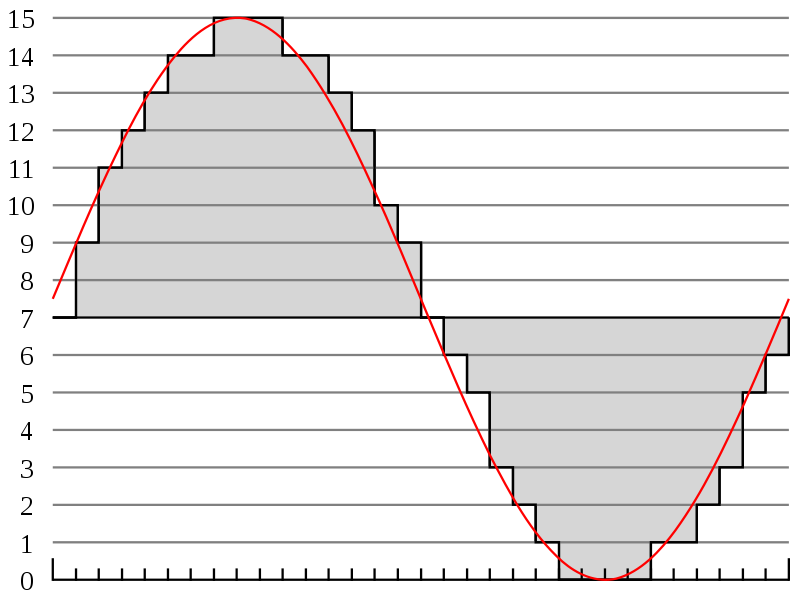
\includegraphics[width=8.098cm,height=6.073cm]{IC2020Codificacion20de20datos-img4.png}

\end{minipage}
\end{center}

\bigskip

\subsubsection{Archivos}
Una vez que se ha obtenido la secuencia de bytes que representa la
información, ya se trate de texto, de multimedia o de otros tipos de
datos, si no queremos perder esta información necesitamos guardarla
en algún medio de almacenamiento permanente, como un disco rígido,
o un pendrive, creando un \textbf{archivo.} Este archivo \textbf{es
precisamente esa secuencia de bytes}, almacenados en algún medio de
almacenamiento.

El archivo, que contiene y transporta nuestra información, ocupará
una cierta cantidad de bytes en ese medio de almacenamiento, y,
dependiendo de la información que guarda, puede tratarse de grandes
cantidades de bytes. Si, por ejemplo, se trata de una imagen de muy
alta \textbf{resolución} (donde la cuadrícula de digitalización
es sumamente fina) y con gran \textbf{profundidad de color} (donde los
colores son representados con muchos valores discretos, necesitando
muchos bytes), entonces la imagen digitalizada será más grande. Es
típico que las cámaras digitales modernas entreguen imágenes
digitales con una resolución de decenas de millones de puntos o
\textbf{pixels}\footnote{\url{http://es.wikipedia.org/wiki/Pixel}},
y estas imágenes suelen ser de muy gran
tamaño\footnote{\url{http://www.360cities.net/london-photo-es.html}:
¡Una fotografía panorámica de miles de millones de pixels! }.

\subsubsection[Múltiplos del bit y del byte]{Múltiplos del bit y del
byte}
Para manejar con comodidad esas grandes cantidades de bits y de bytes
recurrimos a múltiplos, tal como se hace habitualmente con los metros
para grandes distancias (en cuyo caso hablamos de kilómetros, u otras
unidades), o con los gramos para grandes pesos (en cuyo caso hablamos
de kilogramos, u otras unidades). 

Hay dos sistemas de múltiplos de bits y bytes en uso, y a veces esto
causa confusión: el Sistema Internacional (SI) y el sistema de
Prefijos Binarios.

\paragraph{Sistema Internacional (SI)}
El \textbf{Sistema Internacional (SI)}\footnote{\url{http://es.wikipedia.org/wiki/Sistema_Internacional_de_Unidades\#Tabla_de_m.C3.BAltiplos_y_subm.C3.BAltiplos}} 
define múltiplos para todas las unidades de medida. Estos múltiplos
se denominan mediante prefijos que acompañan a la unidad fundamental
de cada magnitud (como, por ejemplo, \textbf{kilo} acompaña a
\textbf{gramo} para crear el múltiplo \textbf{kilogramo}). En el SI,
estos prefijos corresponden a múltiplos elegidos como potencias de
10. Los múltiplos que suelen ser más interesantes para las ciencias
y las ingenierías corresponden a aquellas potencias de 10 cuyo
exponente es múltiplo de 3 (como 10\textsuperscript{3}, 10\textsuperscript{6},
10\textsuperscript{9}...).

Por ejemplo, 10\textsuperscript{3} (que es igual a 1000) se asocia con
el prefijo \textbf{kilo} y se simboliza \textbf{k}, de modo que
kilogramo significa mil gramos y se escribe 1 kg. Del mismo modo,
10\textsuperscript{6} recibe el prefijo \textbf{mega} (simbolizado por \textbf{M}),
10\textsuperscript{9} recibe el prefijo \textbf{giga} (simbolizado por \textbf{G}),
y 10\textsuperscript{12} recibe el prefijo
\textbf{tera} (simbolizado por \textbf{T}). De esta manera, \textbf{un
millón de bytes }se indica como \textbf{1 megabyte} y se escribe
\textbf{1MB}.

\paragraph{Prefijos Binarios}
Sin embargo, en computación es habitual medir la información con
otros múltiplos que no son potencias de 10 sino potencias de 2. Por
ejemplo, para ciertos usos es conveniente considerar los bytes en
conjuntos de 1024 (que es 2\textsuperscript{10}) y no en conjuntos de
1000 (que es 10{\textthreesuperior}). Por este motivo una
organización de estándares, la \textbf{IEC}, creó un conjunto de
múltiplos basados en \textbf{Prefijos
Binarios}\footnote{\url{http://es.wikipedia.org/wiki/Prefijo_binario}}.
Estos múltiplos son cantidades que tienen tamaños similares a los
múltiplos del SI y son simbolizados con las mismas letras, pero son
potencias de 2 cuyo exponente es múltiplo de 10 (como
2\textsuperscript{10}, 2\textsuperscript{20},
2\textsuperscript{30}...). Para construir los prefijos del sistema de
Prefijos Binarios, se agrega la sílaba \textbf{bi} luego de la
primera sílaba del prefijo SI que los representa.

Así, la unidad binaria más cercana al kilobyte (kB) es el
\textbf{Kibibyte} (\textbf{KiB}), que vale 2\textsuperscript{10} bytes
(o sea, 1024 bytes, y no 1000). La unidad binaria más cercana al
megabyte (MB) es el \textbf{Mebibyte} (\textbf{MiB}) que vale
2\textsuperscript{20} bytes (o sea, 1048576 bytes, y no exactamente un
millón). La unidad binaria más cercana al gigabyte (GB) es el
\textbf{Gibibyte} (\textbf{GiB}) que vale 2\textsuperscript{30} bytes
(1073741824 bytes, y no exactamente mil millones). Existen otros
múltiplos mayores, que por el momento no tienen uso diario, pero que
de acuerdo con las tendencias tecnológicas, iremos encontrando con
mayor frecuencia en el futuro cercano (\textbf{Tera, Peta, Exa, Zetta,
Yotta...}). \ 

En computación se utilizan, en diferentes situaciones, ambos sistemas
de unidades, porque es costumbre usar el SI para hablar de
\textbf{velocidades de transmisión de datos}, pero usar Prefijos
Binarios al hablar de \textbf{almacenamiento}. Así, cuando un
proveedor de servicios de Internet ofrece un enlace de \textbf{1Mbps},
nos está diciendo que por ese enlace podremos transferir
\textbf{exactamente 1 millón de bits por segundo}. Por el contrario,
los fabricantes de \textbf{medios de almacenamiento} (como memorias,
discos rígidos o pendrives) acostumbran hablar en términos de
múltiplos binarios, y por lo tanto deberían (aunque normalmente no
lo hacen) utilizar \textbf{Prefijos Binarios} para expresar las
capacidades de almacenamiento de esos medios. Así, un
{\textquotedblleft}pendrive de cuatro gigabytes{\textquotedblright},
que normalmente tiene una capacidad de 4 * 2\textsuperscript{30} bytes,
debería publicitarse en realidad como {\textquotedblleft}pendrive de
cuatro Gibibytes{\textquotedblright}. 

\subsubsection{Compresión}
Muchas veces es interesante reducir el tamaño de un archivo, para que
ocupe menos espacio de almacenamiento o para que su transferencia a
través de una red sea más rápida. Al ser todo archivo una
secuencia de bytes, y por lo tanto de números, disponemos de
métodos y herramientas matemáticas que permiten, en ciertas
condiciones, reducir ese tamaño. La manipulación de los bytes de un
archivo con este fin se conoce como \textbf{compresión.}

La compresión de un archivo se ejecuta mediante un programa que
utiliza un algoritmo especial de compresión. Este algoritmo puede ser
de \textbf{compresión sin pérdida, o con
pérdida}\footnote{\url{http://es.wikipedia.org/wiki/Digitalización\#Compresión}}.

\paragraph{Compresión sin pérdida}
Decimos que la compresión ha sido sin pérdida cuando, del archivo
comprimido, puede extraerse exactamente la misma información que
antes de la compresión, utilizando otro algoritmo que ejecuta el
trabajo inverso al de compresión. En otras palabras, la compresión
sin pérdida es \textbf{reversible}: siempre puede volverse a la
información de partida. Esto es un requisito indispensable cuando
necesitamos recuperar exactamente la secuencia de bytes original, como
en el caso de un archivo de texto. Como usuarios de computadoras, es
muy probable que hayamos utilizado más de una vez la compresión sin
pérdida, al tener que comprimir un documento de texto que nosotros
hicimos utilizando un programa utilitario como
ZIP\footnote{\url{http://es.wikipedia.org/wiki/Formato\_de\_compresión\_ZIP}},
RAR u otros. Si la compresión no fuera reversible, no podríamos
recuperar el archivo de texto tal cual lo escribimos.

\paragraph{Compresión con pérdida}
En algunos casos, el resultado de la compresión de un archivo es otro
archivo del cual \textbf{ya no puede} \textbf{recuperarse} la misma
información original, pero que de alguna manera sigue sirviendo a los
fines del usuario. Es el caso de la compresión de imágenes, donde
se reduce la calidad de la imagen, ya sea utilizando menos colores, o
disminuyendo la resolución. También es el caso de la compresión
de audio, al descartar componentes del sonido con frecuencias muy bajas
o muy altas, inaudibles para los humanos (como en la tecnología de
grabación de CDs), con lo cual la diferencia entre el original
digital y el comprimido no es perceptible al oído. También es
útil, para algunos fines, reducir la calidad del audio quitando
componentes audibles (lo que hacen, por ejemplo, algunos grabadores
{\textquotedblleft}de periodista{\textquotedblright} para lograr
archivos más pequeños, con audio de menor fidelidad, pero donde el
diálogo sigue siendo comprensible).
\end{document}
